\thispagestyle{empty}
\subsection*{\huge Summoner}
\vspace{0.3cm}
"I don’t like your plan. It sucks." \\
\indent -- Yuna 
\vspace{0.3cm} \\
Summoners are powerful spellcasters that can summon magical beasts to aid them in combat. 
They create a strong bond to their summon allowing the summoner to control their incredible powers to his
will. 
While the summoners themselves focus on using defensive magic, their summons can wreak havoc unlike any human being.
\vfill
\battrt{
	\textbf{Level 1:} & HP +16 & MP~+19 & AGI~+2 & MAG~+1 \\ 
	\textbf{Level 2:} & HP~+5  & MP~+10 & RES~+1 & STR~+1 \\ 
	\textbf{Level 3:} & HP~+10 & MP~+10 & MAG~+1 &         
}{Staff}{Robe}
\vfill
\atypet{Devout}
{	
	\textbf{Level 4:} & HP~+5  & MP~+10 & RES~+1 & DEF~+1 \\  
	\textbf{Level 5:} & HP~+10 & MP~+10 & MAG~+1 &        \\  
	\textbf{Level 6:} & HP~+5  & MP~+10 & MAG~+1 & RES~+1 \\  
	\textbf{Level 7:} & HP~+5  & MP~+10 & RES~+2 &        \\  
	\textbf{Level 8:} & HP~+10 & MP~+10 & DEF~+1 &		  \\  
	\textbf{Level 9:} & HP~+5  & MP~+10 & MAG~+1 & RES~+1 \\  
	\textbf{Level 10:}& HP~+10 & MP~+10 & MAG~+1 &        \\  
}
{Soulbind}
{	
	On your turn, your currently active summon can cast a spell where he can spend your MP in addition to his own and the spell's cast time is reduced by 1 round.
	You have to skip your own turn to use this effect.
}
{Sacrifice}
{	
	Whenever your currently active summon would receive any damage, you can choose to reduce your own HP by the same amount instead.
}
\vfill
\atypet{Evoker}
{		
	\textbf{Level 4:} & HP~+10 & MP~+5  & MAG~+1 & DEF~+1 \\  
	\textbf{Level 5:} & HP~+10 & MP~+10 & RES~+1 &		  \\  
	\textbf{Level 6:} & HP~+5  & MP~+10 & MAG~+1 & RES~+1 \\  
	\textbf{Level 7:} & HP~+10 & MP~+5  & DEF~+1 & RES~+1 \\  
	\textbf{Level 8:} & HP~+5  & MP~+10 & MAG~+2 &	      \\  
	\textbf{Level 9:} & HP~+5  & MP~+10 & RES~+1 & MAG~+1 \\  
	\textbf{Level 10:}& HP~+10 & MP~+10 & RES~+1 &		  \\  
}
{Channel}
{	
	On your turn, you can choose to cast a spell known by your currently active summon and the spell's cast time is reduced by 1 round. 
	The summon has to skip his turn to you use this effect.
}
{Lifesiphon}
{	
	Whenever you would receive any damage, you can choose to reduce the HP of your currently active summon by the same amount instead.
}
\pagebreak \\
\noindent {\Large\color{accent}\bf \uline{Abilities\phantom{y}\hfill}}\\\\
\spellt{Summon}{8}{3r}{Single}{Self}
{
	You summon a creature that acts with you on your turn, following your command.
	The summon is dismissed when you or the summon suffers \hyperlink{status}{KO}, but you can also dismiss it whenever you want.
	Once dismissed, you cannot summon the same creature again on the same day.
	All creatures that you can summon at different Levels are shown on the next page.
}{}{1}
\spellt{Pray}{5}{1r}{1u}{Self}{
	Everyone in the target area regains 1d HP. 
}{}{2}
\spellt{Image}{10}{1r}{1u}{3u}{
	The target gains \hyperlink{status}{Blink} for 3 rounds.
}{\blink}{4}
\spellt{Toad}{16}{1r}{Single}{3u}{
	The target makes a DC 8 check and is turned into a toad upon failure for 3 rounds or until he receives any damage.
	While being a toad, the target cannot talk or take any action and can only move 1u per turn.
}{}{6}
\spellt{Dispel}{20}{1r}{Single}{3u}{
	All \hyperlink{type}{Resiliences} and \hyperlink{status}{Immunities} of the target are removed for 3 rounds.
	Also, all beneficial \hyperlink{status}{Status Effects} that are active on the target when this spell takes effect are completely removed as well.
}{}{8}
\spellt{Twin Summon}{28}{5r}{Single}{Self}{
	You summon two different creatures that both follow your command and act with you on your turn.
	The summons are dismissed when you or they suffer \hyperlink{status}{KO}, but you can also dismiss them whenever you want.
	Once dismissed, you cannot summon the same creature again on the same day.
	All creatures that you can summon at different Levels are shown on the next page. 
}{}{10}
\vspace{5cm}
\pagebreak
\onecolumn
\noindent{\LARGE\color{accent}\bf \uline{Summons\hfill} \\} \\
\thispagestyle{empty}

\begin{multicols}{2}
\friendly{Carbuncle}{1}{
\includegraphics[width=0.18\textwidth]{./art/monsters/carbuncle.png}}
{
	HP: & \hfill 20 & MP: & \hfill 36\\
	STR: & \hfill 1 & DEF: & \hfill 0 \\
	MAG: & \hfill 2 & RES: & \hfill 2 \\
	AGI: & \hfill 3 & Size: & \hfill S\\
}
{
	\textbf{Tackle}: 1d DMG\phantom{y} 
	
	\mspell{Reflect}{12}{1r}{Single}{3u}{The target gains a shield that reflects the next spell that targets them back to its caster.}{}		
}
\vspace{0.5cm} 
\friendly{Ifrit}{3}{
\includegraphics[width=0.23\textwidth]{./art/monsters/ifrit.png}}
{
	HP: & \hfill 50 & MP: & \hfill 36\\
	STR: & \hfill 2 & DEF: & \hfill 3 \\
	MAG: & \hfill 1 & RES: & \hfill 0 \\
	AGI: & \hfill 3 & Size: & \hfill M\\
}
{
	\textbf{Claw}: 2d DMG \\
	\textbf{Resilience}:\fire \hfill \textbf{Weakness:}\ice
	
	\mspell{Fire}{4}{1r}{Single}{3u}{You deal 2d \hyperlink{fire}{fire} damage to the target.}{\fire}	
	\mtech{Hellfire}{12}{1r}{2u}{Self}{You deal 4d \hyperlink{type}{fire} damage to everyone in the target area except yourself.}{\fire}	
}
\vspace{0.5cm} 
\friendly{Shiva}{5}{
\includegraphics[width=0.18\textwidth]{./art/monsters/shiva.png}}
{
	HP: & \hfill 60 & MP: & \hfill 80\\
	STR: & \hfill 1 & DEF: & \hfill 1 \\
	MAG: & \hfill 5 & RES: & \hfill 4 \\
	AGI: & \hfill 3 & Size: & \hfill M\\
}
{
	\textbf{Icicle}: 2d DMG, 3u Range \\
	\textbf{Resilience}:\ice \hspace*{\fill} \textbf{Weakness:}\fire
	
	\mspell{Deprotect}{5}{1r}{Single}{3u}{The target suffers \hyperlink{status}{DeDEF} for 3 rounds.}{\dedef}
	\mspell{Deshell}{5}{1r}{Single}{3u}{The target suffers \hyperlink{status}{DeRES} for 3 rounds.}{\deres}
	\mtech{Ice Wall}{10}{1r}{3u (line)}{3u}{
	You create a 3u tall and wide wall of ice that blocks the path for 5 rounds.
	The wall breaks down after 3 rounds or upon suffering a total of 30 damage.
	}{}
	\mspell{Diamond Dust}{20}{1r}{3u (front)}{Self}{
	All enemies in the target area suffer 6d \hyperlink{type}{ice} damage and \hyperlink{status}{Immobile} for 1 round.	
	}{\ice\immobile}		
}
\friendly{Phoenix}{7}{
\includegraphics[width=0.2\textwidth]{./art/monsters/phoenix.png}}
{
	HP: & \hfill 70 & MP: & \hfill 90\\
	STR: & \hfill 0 & DEF: & \hfill 2 \\
	MAG: & \hfill 6 & RES: & \hfill 8 \\
	AGI: & \hfill 2 & Size: & \hfill M\\
}
{
	\textbf{Beak}: 1d DMG  \\ 
	\textbf{Immune}: \hyperlink{status}{All Status Effects} \hfill \textbf{Resilience:}\fire\holy
	
	\mspell{Protect}{5}{1r}{Single}{3u}{The target gains \hyperlink{status}{EnDEF} for 3 rounds.}{\enndef}
	\mspell{Shell}{5}{1r}{Single}{3u}{The target gains \hyperlink{status}{EnRES} for 3 rounds.}{\enres}
	\mspell{Curaga}{18}{1r}{1u}{3u}{Everyone in the target area regains 6d HP.}{}
	\mspell{Full-Life}{28}{3r}{Single}{3u}{Remove \hyperlink{status}{KO} from the target and fully heal his HP.}{\ko}	
	
}
\vspace{0.5cm} 
\friendly{Bahamut}{9}{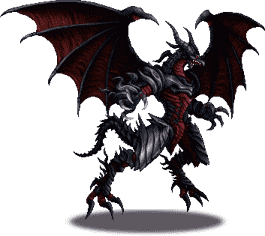
\includegraphics[width=0.23\textwidth]{./art/monsters/bahamut.png}}
{
	HP: & \hfill 100 & MP: & \hfill 140\\
	STR: & \hfill 8 & DEF: & \hfill 6 \\
	MAG: & \hfill 7 & RES: & \hfill 4 \\
	AGI: & \hfill 4 & Size: & \hfill L\\
}
{
	\textbf{Claw}: 3d DMG, 2u Range \\
	\textbf{Immune}: \hyperlink{status}{All Status Effects} \hfill \textbf{Resilience:}\dark 

	\mtech{Obliterating Breath}{20}{1r}{3u (front)}{3u}{
	Everyone in the target area makes a DC 8 check and suffers 4d damage as well as \hyperlink{status}{Poison} and \hyperlink{status}{Blind} for 3 rounds upon failure.
	}{\poison \blind}
	\mspell{Banish}{30}{1r}{Single}{3u}{
	The target makes a DC 8 check and upon failure he is banished into another dimension and thus removed from the battlefield for 3 rounds.
	}{}
	\mspell{Megaflare}{40}{3r}{Single}{8u}{
		You deal 10d+20 \hyperlink{type}{fire} damage to the target.
	}{\fire}
	\mreaction{Final Attack}{If you are about to fall to 0 HP you may use one of your abilities without cost or cast time before falling \hyperlink{status}{KO}.}	
}
\end{multicols}
\twocolumn